% Authoritative TeX source. Conceptual execution diagram; no simulated trace.
\documentclass[border=0pt]{standalone}
% Adapted from tikz-scientific-figures/assets/preamble.tex.
\usepackage{tikz}
\usepackage{pgfplots}
\usepackage{amsmath}
\pgfplotsset{compat=1.18}
\usetikzlibrary{calc,plotmarks}
% Okabe--Ito palette, with shapes and dash patterns for grayscale reading.
\definecolor{cbBlue}{RGB}{0,114,178}
\definecolor{cbGreen}{RGB}{0,158,115}
\definecolor{cbVermillion}{RGB}{213,94,0}
\definecolor{cbPurple}{RGB}{204,121,167}
\definecolor{cbBlack}{RGB}{60,60,60}
\tikzset{
 cstyle/.style={cbBlack,dashed,line width=.65pt,mark=square,mark size=1.65pt,mark options={solid,fill=white}},
 fstyle/.style={cbVermillion,line width=.95pt,mark=*,mark size=1.8pt},
 fanstyle/.style={cbBlue,densely dotted,line width=.85pt,mark=diamond,mark size=2pt,mark options={solid,fill=white}},
 mstyle/.style={cbBlue,densely dotted,line width=.85pt,mark=diamond,mark size=2pt,mark options={solid,fill=white}},
 rstyle/.style={cbPurple,dashdotted,line width=.75pt,mark=triangle,mark size=2pt,mark options={solid,fill=white}},
 nstyle/.style={cbBlue,line width=.7pt,mark=triangle,mark size=2pt,mark options={solid,fill=white}},
 astyle/.style={cbGreen,dashdotted,line width=.7pt,mark=diamond*,mark size=1.75pt},
 acstyle/.style={cbPurple,only marks,mark=x,mark size=2.5pt,line width=.85pt}
}
\pgfplotsset{paperaxis/.style={
 scale only axis,font=\fontsize{8}{9.2}\selectfont,
 tick label style={font=\fontsize{8}{9.2}\selectfont},
 label style={font=\fontsize{8}{9.2}\selectfont},
 y label style={at={(axis description cs:-.28,.5)},xshift=2.5mm},
 line width=.45pt,tick style={line width=.4pt},tick align=outside,
 grid=major,grid style={black!13,line width=.25pt},
 scaled ticks=false,xticklabel style={/pgf/number format/1000 sep={}},
 yticklabel style={/pgf/number format/1000 sep={}},
 enlarge x limits=false,enlarge y limits=false,
 axis on top=false,clip=true
}}

\usetikzlibrary{arrows.meta,positioning}
% ===== TUNABLES: physical size, font, colors =====
\def\figwidth{174mm}
\def\figheight{57mm}
\begin{document}
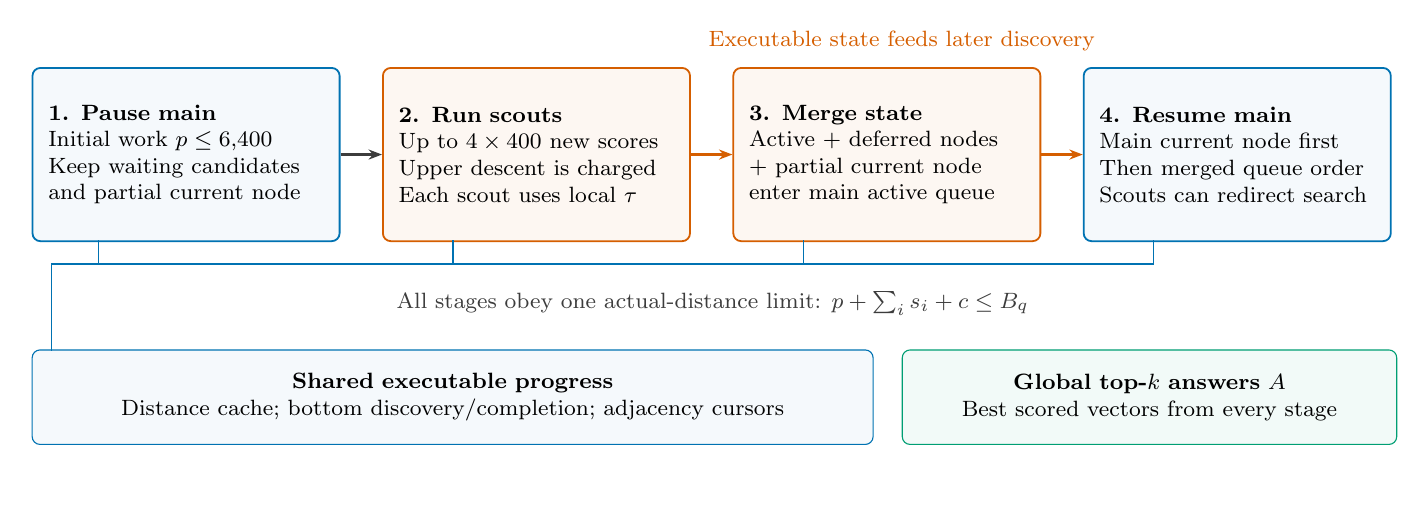
\begin{tikzpicture}[x=1mm,y=1mm,font=\fontsize{8}{9.6}\selectfont,
 stage/.style={draw=cbBlue,line width=.65pt,rounded corners=1mm,fill=cbBlue!4,align=left,text width=35mm,inner sep=2mm,minimum height=22mm},
 arr/.style={-{Stealth[length=1.7mm]},line width=.8pt,cbBlack}]
\path[use as bounding box] (0,0) rectangle (\figwidth,\figheight);
\node[stage,anchor=north west] (main) at (0.5,52) {\textbf{1. Pause main}\\Initial work $p\leq6{,}400$\\Keep waiting candidates\\and partial current node};
\node[stage,anchor=north west,draw=cbVermillion,fill=cbVermillion!5] (scout) at (45,52) {\textbf{2. Run scouts}\\Up to $4\times400$ new scores\\Upper descent is charged\\Each scout uses local $\tau$};
\node[stage,anchor=north west,draw=cbVermillion,fill=cbVermillion!5] (merge) at (89.5,52) {\textbf{3. Merge state}\\Active + deferred nodes\\+ partial current node\\enter main active queue};
\node[stage,anchor=north west] (resume) at (134,52) {\textbf{4. Resume main}\\Main current node first\\Then merged queue order\\Scouts can redirect search};
\draw[arr] (main.east) -- (scout.west);
\draw[arr,cbVermillion] (scout.east) -- (merge.west);
\draw[arr,cbVermillion] (merge.east) -- (resume.west);
\node[align=center,text=cbBlack] at (87,22) {All stages obey one actual-distance limit: $p+\sum_i s_i+c\leq B_q$};
\node[draw=cbBlue,fill=cbBlue!4,rounded corners=1mm,anchor=south west,
 align=center,text width=104mm,minimum height=12mm,inner sep=1.4mm] (shared) at (0.5,4)
 {\textbf{Shared executable progress}\\Distance cache; bottom discovery/completion; adjacency cursors};
\node[draw=cbGreen,fill=cbGreen!5,rounded corners=1mm,anchor=south west,
 align=center,text width=60mm,minimum height=12mm,inner sep=1.4mm] (answers) at (111,4)
 {\textbf{Global top-$k$ answers $A$}\\Best scored vectors from every stage};
\draw[cbBlue,line width=.55pt] (9,30) -- (9,27) -- (3,27) -- (3,16);
\draw[cbBlue,line width=.55pt] (54,30) -- (54,27) -- (9,27);
\draw[cbBlue,line width=.55pt] (98.5,30) -- (98.5,27) -- (54,27);
\draw[cbBlue,line width=.55pt] (143,30) -- (143,27) -- (98.5,27);
\node[anchor=south,inner sep=0pt,text=cbVermillion] at (111,54) {Executable state feeds later discovery};
\end{tikzpicture}
\end{document}
